\chapter{Prescriptive Analysis for steam injection optimization}

\section{Introduction}
Steam Flooding is a thermal oil recovery method. In this method, steam forms a condensing zone inside the reservoir. The heat of condensation is utilized to heat up the heavy crude oil, facilitating its displacement due to a reduction in viscosity (Ali and Meldau 1979). The injected steam forms a steam chamber around the injection well as shown in Fig. \ref{fig:steam_process} (Zhang and Chen 2018). The steam chamber is expanded towards the production well. The condensed water displaces the reservoir fluid into the production well (Shafiei and Dusseault 2013; Zhang and Chen 2018).

 \begin{figure}
     \centering
     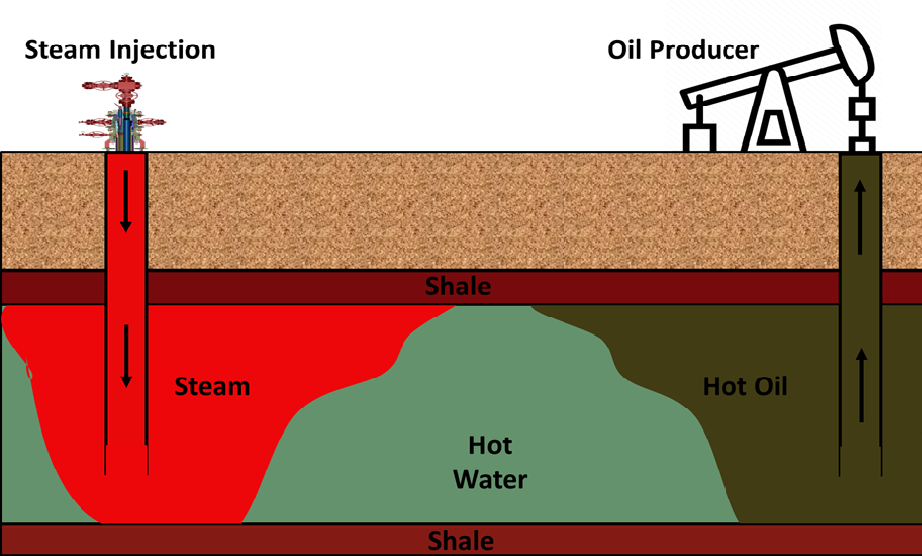
\includegraphics[width = \textwidth]{figures/prescriptive_analysis/steam_process.png}
     \caption{Steam Injection process}
     \label{fig:steam_process}
 \end{figure}
 
Because of the high steam cost, one of the necessary objectives in steam injection projects is the dynamic injection rates optimization. Due to reservoir simulation complexity involved in the steam injection, there is no single steam injection rate value can be optimum for all steam flooding situations. Also, It is difficult for engineers to find a strategy to inject steam over the entire production horizon that maximizes the net present value. Hence, there are some attempts in the literature to optimize steam injection rates. These attempts can be divided to two groups. The first which deals with the steam injection as a steady state problem that means such researches would provide only one single value of injection rate as an optimum value along the production horizon. Others, will study the problem as a dynamic optimization problem where the output would be an injection rate strategy over time.  

Both optimization solutions would have the objective of maximizing cumulative performance of the wells. The first group includes evolutionary algorithms such as non-dominated sorting genetic algorithm and particle swarm optimization algorithm to optimize injection rate. (Ameli and Mohammadi 2018) applied particle swam optimization, genetic algorithm and imperialist competitive algorithm in order to optimize steam to oil ratio. Their results should that GA worked 6% better in comparison to other optimization techniques and it was also faster in comparison to continuous optimization algorithm. As aforementioned the biggest drawback of that approach is that it only provides a single value for steam injection or steam ration that is not sufficient in such a complex problem. 

On the hand, the second group of researches deal with steam injection as an optimal control problem. This group of researches include the model predictive control algorithm and the adjoint based method. Model Predictive Control (MPC) is considered the most widely used advanced control method in refining, chemical, and petrochemical processes (Saputelli et al. 2005; Patel et al. 2014; Purkayastha et al. 2015; Eaton et al. 2017; Vembadi et al. 2018). MPC is a control algorithm that is built on the concept of moving horizon. For the steam injection problem, a proxy model is introduced to formulate the problem. This proxy model is a relation between injection rates and oil and water production rates.  Finally, the formulated problem is optimized over the prediction horizon to find the steam injection rates that maximize the net present value. However MPC approach is preferable but the drawback of combining with proxy model to formulate the system makes it unstable and only suitable for small horizon of production (Sibaweihi et al. 2021). 

In the second group also lies the adjoint-method. It is perform some sort of gradient-based optimization method where the derivatives are obtained through the use of an adjoint equation or co-state equation (Giannakoglou and Papadimitriou 2008; Zhang et al. 2014). It depends on the barrier function to formulate the augmented objective function. Hence, the augmented objective function includes the calculation of net present value and the constraints that formulate the reservoir dynamics. The disadvantage of this approach is that the equations representing the gradient of the augmented objective function with respect to the steam injection rate must be hard-coded which is not easy in case of thermal oil recovery processes where compositional models are used (Guevara et al. 2021). 
More recent applications in the area of complex control included the application of reinforcement learning (RL) (Mullapudi et al. 2020; Siraskar 2021; Garnier et al. 2021). In RL, a learner and decision maker called agent is trained to find the optimal policy. 

Some examples of the use of RL include, among others, the abstract-strategy games (Vinyals et al. 2017; Germain and Marfoq 2019), the real-time traffic signal control (Abdulhai et al. 2003; S. El-Tantawy and B. Abdulhai 2012), the optimization of energy conservation and comfortable temperatures in buildings (Dalamagkidis et al. 2006) and the autonomous control of vehicles (Folkers et al. 2019). 

In the field of subsurface energy management, RL applications are found in the context of guided drilling control of oil and gas wells (Liu et al. 2018; ArnØ et al. 2020; Yu et al. 2021), waterflooding optimization Projects (Ma et al. 2019; Hourfar et al. 2019; Miftakhov et al. 2020), CO2 storage (Sun 2020), SAGD (Guevara et al. 2021), optimal well placement and well type selection (De Paola et al. 2020; Dawar 2021) and in the area of pressure transient tests interpretation (Dong et al. 2022).

(Guevara et al. 2021) have proposed the usage of reinforcement learning to address the problem of steam assisted gravity drainage. Their methodology included the application of state-action-reward-state-action (SARSA). It is an on-policy reinforcement learning algorithm that estimates the value of the policy being followed. SARSA learns a near-optimal policy whilst exploring. Unlike SARA, actor critic reinforcement learning algorithm evaluate and enhance to the policy therefore the agent continue updating the policy and exploring till learning optimal policy. Whereas On-Policy learns suboptimal policy. In addition, actor-critic methods combine advantages of value-based and policy-based approaches. In this algorithm, the actions generated by a policy neural network. This network is evaluated based on a corresponding change in state potential. These values are given by another neural network called the critic network. This network approximates the expected cumulative reward from the given state (Thuerey et al. 2022).

In this work, a model free  reinforcement learning (RL) is applied for steam injection rate optimization. it was selected because it overcomes the shortcomings of the aforementioned methods in two points. Firstly, it does not require a full description of the process required to be optimized. Secondly, this approach takes advantage of previous experiences or the interactions with the environment to find an optimal policy of injection rate to maximize the net present value without human interference. 


\section{Elements of \ac{RL}}

\ac{RL} technique is the preferred method for the purpose of this paper. It is highlighted because the optimal policy (policy that maximizes the reward of the decision process). Hence, it supports automated transformation and going beyond conventional approaches to solve the task at hand. Reinforcement learning problems involve learning how to map situations to actions in a closed-loop structure where the learning system’s actions influence its later inputs converging towards the maximum numerical reward signal. Moreover, the learner discover which actions yield the best reward by trying them out. Fig 2 presents the agent-environment interaction in the reinforcement learning.

 \begin{figure}
     \centering
     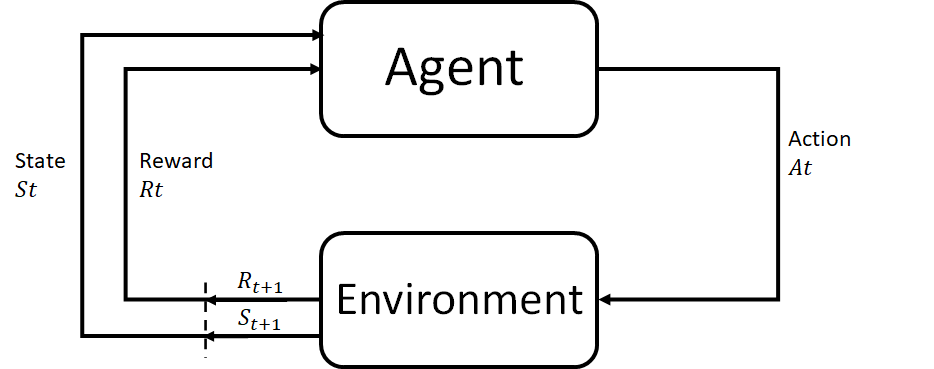
\includegraphics[keepaspectratio, width =\textwidth]{figures/prescriptive_analysis/rl.png}
     \caption{The agent-environment interaction in \ac{RL}}
     \label{fig:rl}
 \end{figure}
 
Figure \ref{fig:rl} The agent-environment interaction in RL
In a challenging environments, actions may affect not only the immediate reward but also the next situation and therefore all subsequent rewards. To conclude, there are three main features of RL that make it the preferred option: to being closed-loop in an essential way, not to having direct instructions as to what actions to take, and where the consequences of actions, including reward signals,  and to fluctuate actions over extended time periods (Sutton and Barto 2005).

\subsection{Environment}
„Environment“ is a mathematical model that mimics the behaviour of the environment. In other words, it presents inferences of how the environment behaves. For instance, the model might predict the resultant next state st+1 and next reward rt+1 given a state st and taking action at. 

\subsection{Reward function}
A reward signal is considered the target or the objective function in a reinforcement learning problem. It is a single number sent from the environment to the reinforcement learning agent at any time depends on the agent’s current action and the current state of the environment. The agent can influence the reward signal is through its action. Therefore, Maximizing the total reward that the agent receives over the long run is considered its main objective. The reward signal defines the good and bad actions for the agent. It is denoted by $R_t$ at time step (t).

\subsection{Value function}
A value function is used to evaluate the success on the long run. Roughly speaking, the value of a state, i.e. the status of the agent: what has been learned – what must be done, is the total amount of rewards an agent can expect to accumulate over the future, starting from a specific state at time (t), which can for instance  be the   initial conditions of the simulations  towards the end of the episode. Whereas reward determines the immediate return at a specific environmental state, function value indicate the long-term desirability of state after considering the states that are likely to follow. In other words, the value function at state (s) considers the reward available in (s) and the upcoming states. The Value function is denoted by $\pi$ where $V_\pi(S)$ is the value function for a given a specific state (S) under a specific policy $\pi$.

\subsection{Policy function}
A policy defines the learning agent’s way of behaving at a given time. Roughly speaking, a policy can be considered as an interconnection between states (The Input vector from the environment at a specific time step t) and actions (what should be done?). The policy is denoted $\pi_t$ where $\pi_t\left(a|s\right)$ is the probability of taking an action $(a)$ when being in certain state $(s)$.

\subsection{Learning Dynamics (Agent-Environment interactions)}

Over a sequence of discrete time steps $t = {0, 1, 2, 3, …, T}$, an agent interacts with an environment E. In every iteration, the agent receives a current state from the environment $(st)$ and selects an action from some set of possible actions $(a)$ according to its policy $pi$. In return, the agent receives the next state $s_t+1$ and receives a scalar reward $r_t$. The process continues until either the agent reaches a terminal state or the maximum number of time steps satisfied after which the process restarts (Bilgin 2020).

The total accumulated return from time step t can be calculated from $R_t=\ \sum_{k=0}^{\infty}{\gamma^k{\ r}_{t+k}}$ were $\gamma \in [0, 1]$ is the discount factor. The value of state $s$ under policy $pi$ is defined as $V_pi(s) = \mathbb{E}\left[R_t|s_t = s\right]$ and is simply the expected return for following policy $pi$ from state $s$. Another important function while learning is the action value function $Q_pi(s, a) = \mathbb{E}\left[R_t|s_t\right]$. It is the expected yield for a specific action a at a state s and following policy $pi$. 

Solving a reinforcement learning task means reaching the optimal policy. It is the one that going to give us the maximum value in any state we are in $\pi^\ast= argmax_\pi \mathbb{E}_\pi\sum_{k=0}^{\infty}{\gamma^k{\ r}_{t+k}}$. There are two techniques to solve the problem in model free reinforcement learning either value based technique or policy based technique.

In value-based model-free reinforcement learning methods, There is no explicit policy is stored but only solving the problem of the value function. The policy is here implicit and can be derived directly from the value function by picking the action with the best value. For instance DQN is the most popular Q-learning algorithm. In this algorithm, the action value function is represented using a function approximator, such as a neural network $Q(s,\ a;\ \theta)$. The objective is to directly approximate the optimal action value function: $Q\ast(s,\ a)\ \approx\ Q(s,\ a;\ \theta)$. The learning is done iteratively through continuous update of the parameters $\theta$ of the action value function minimizing a sequence of loss functions.

Equation \ref{Eq:rl_loss} shows the loss function applied per iteration $i$.

\begin{equation} \label{Eq:rl_loss}
J(\theta_i)\ =\ \mathbf{E}{(r+\ \gamma\max\below{a^,}{Q(s^,,a^,,\theta_{i-1})-Q(s,a,\theta_i)})}^2
\end{equation}

where $s^$, is the state at $t+1$ after state $s$ at time $t$. 

On the contrary, we explicitly build a parameterized representation of the policy $PI(a_t|s_t; \theta)$ in the policy-based methods. Then, gradient ascent on $\mathbf{E}[R_t]$ is performed to update the parameters $\theta$. An example of such a method is the REINFORCE family of algorithms.

In this algorithm the policy parameters $\theta$ is updated in the direction $\nabla \theta\ log\ \pi(a_t|s_t;\ \theta)\ast R_t$. In order to solve the problem of the high variance of such estimates while keeping it unbiased, A learned estimate of the value function is commonly used as the baseline $bt(st)\ \approx\ V\pi(st)$.  It is commonly known as a baseline. This base line is subtracted from the return. Hence, The resulting gradient is calculated from $\nabla\theta\ log\ \pi(at|st;\ \theta)\ (Rt\ -\ bt(st))$ (Sutton and Barto 2005).

The advantage actor critic reinforcement learning combines both techniques, the value based and the policy based, together. It consists of two neural networks and the advantage function. The later calculates the agent’s TD Error or Prediction Error. The actor network can be considered as a policy gradient algorithm that chooses an action at each time step. On the other hand, the critic network evaluates the Q-value or provide a feedback on how to adjust. While the critic network learns which states are better or worse, the actor uses the critic results to teach the agent to seek out good states and avoid bad states.


\section{Implementation}

\subsection{Environment}
A reservoir simulation model represents our environment. In this case, one-eighth of an inverted nine-spot pattern is used to displace oil by steam (Aziz et al. 1987). The total area of the pattern is 2.5 acres with grid system of 23 x 12 x 12. The case is shown in Fig. \ref{fig:grids}. Grid points are distributed uniformly in the horizontal plane as shown. The well radii for all three wells are 0.3 ft.

\begin{figure}
    \centering
    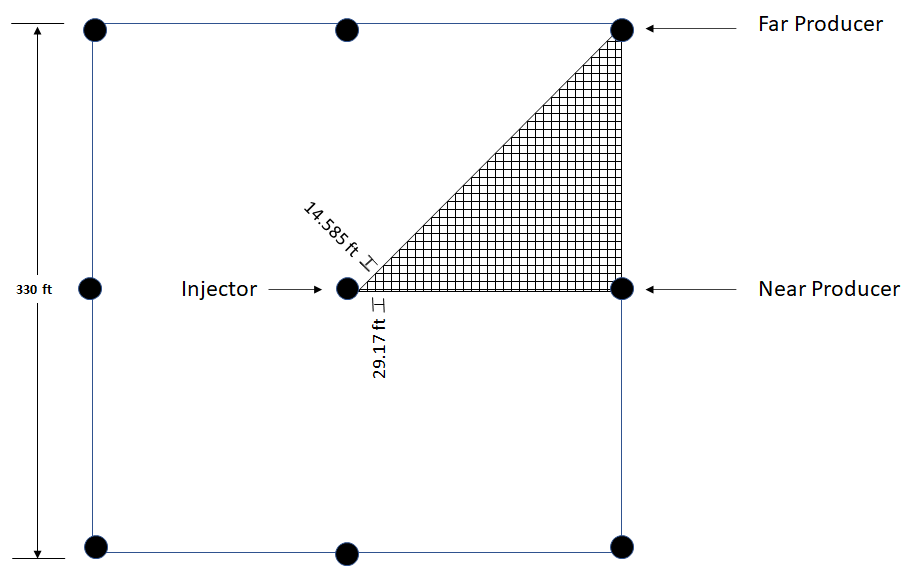
\includegraphics[width = \textwidth]{figures/prescriptive_analysis/grids.png}
    \caption{3 Element of symmetry used in the simulation of steam injection in an inverted nine-spot}
    \label{fig:grids}
\end{figure}
 
Figure \ref{fig:grids} Element of symmetry used in the simulation of steam injection in an inverted nine-spot
Rock Properties:
Vertical permeabilities are 50% of horizontal values. Porosity of all layers is 0.3 (fraction). Thermal conductivity of reservoir overburden and underburden is 24 BTU/(ft-D-OF). Heat capacity of reservoir overburden and underburden is 35 Btu/(ft3 of rock-OF). Effective rock compressibility is 5x 10-4 psi- 1. 


Fluid Properties: 
Properties of pure water are assumed Oil density at standard conditions is 60.68 Ibm/ft3. Compressibility is 5x10-6 psi-1. The coefficient of thermal expansion is 3.8 x 10-4 OR-1, and the molecular weight is 600. Temperature and viscosity data are shown in Table \ref{tab:temp_vis_steam}. Further information about the produced fluid properties and initial oil composition can be found in table \ref{tab:steam_fluid_components} and \ref{tab:steam_fluid_components}.

\begin{table}[]
\center
\begin{tabular}{|l|l|}
\hline
Temperature ($\circ$F) & Viscosity (cp) \\ \hline
75               & 5,780          \\ \hline
100              & 1,380          \\ \hline
150              & 187            \\ \hline
200              & 47             \\ \hline
250              & 17.4           \\ \hline
300              & 8.5            \\ \hline
350              & 5.2            \\ \hline
500              & 2.5            \\ \hline
\end{tabular}
\caption{Temperature and viscosity data}
\label{tab:temp_vis_steam}
\end{table}

\begin{table}[]
\center
\resizebox{0.8\columnwidth}{!}{%
\begin{tabular}{l|lll|}
\cline{2-4} & \multicolumn{3}{l|}{Components}\\ \cline{2-4} & \multicolumn{1}{l|}{1}   & \multicolumn{1}{l|}{2}   & 3   \\ \hline
\multicolumn{1}{|l|}{Molecular weight}         & \multicolumn{1}{l|}{250} & \multicolumn{1}{l|}{450} & 600 \\ \hline
\multicolumn{1}{|l|}{Specific heat, Btu/Ibm-oR}                & \multicolumn{1}{l|}{0.53} & \multicolumn{1}{l|}{0.55}  & 0.6  \\ \hline
\multicolumn{1}{|l|}{Density at standard   conditions Ibm/ft3} & \multicolumn{1}{l|}{52.3} & \multicolumn{1}{l|}{57.64} & 61.2 \\ \hline
\multicolumn{1}{|l|}{Critic   pressure, psia}  & \multicolumn{1}{l|}{225} & \multicolumn{1}{l|}{140} & --  \\ \hline
\multicolumn{1}{|l|}{Critical temperature, oF} & \multicolumn{1}{l|}{800} & \multicolumn{1}{l|}{950} & --  \\ \hline
\end{tabular}%
}
\caption{properties of oil components}
\label{tab:steam_fluid_components}
\end{table}

\begin{table}[]
\center
\begin{tabular}{|l|l|}
\hline
Components & Mole Fraction \\ \hline
C1         & 0.5030        \\ \hline
C2         & 0.1614        \\ \hline
C3         & 0.3356        \\ \hline
\end{tabular}%
\caption{Initial oil Composition}
\label{tab:steam_composition}
\end{table}

Rock-fluids interaction:
For water/oil system, the residual oil saturation (Sorn) is 0.15. For gas/oil system, the residual oil saturation (Sorg) is 0.10. The critical gas saturation (Sgc)  is 0.06.

Regarding permeabilities, the oil relative permeability at interstitial water saturation, kroiw is 0.4. For water/oil system, water relative permeability at residual oil saturation (krwro) is 0.1. For gas/oil system, gas relative permeability at residual oil saturation (krgro) is 0.2. Equations ~\eqref{Eq:relatiperm1}~--~\eqref{Eq:relatiperm4} define the relative permeability for the water/oil system and for the gas/oil system as

\begin{equation}\label{Eq:relatiperm1}
k_{rw}\ =\ k_{rwro}\ \left(\frac{S_w-S_{wir}}{1-S_{orw}-S_{wir}}\right)^{2.5}
\end{equation}

\begin{equation}\label{Eq:relatiperm2}
k_{row}\ =\ k_{roiw}\ \left(\frac{{1-S}_{orw}-S_w}{1-S_{orw}-S_{iw}}\right)^2		
\end{equation}

\begin{equation}\label{Eq:relatiperm3}
k_{rg}\ =\ k_{rgro}\ \left(\frac{S_g-S_{gc}}{1-S_{iw}-S_{gc}}\right)^{1.5}		    
\end{equation}

\begin{equation}\label{Eq:relatiperm4}
k_{rw}\ =\ k_{rwro}\ \left(\frac{1-S_{iw}-S_{org}-S_g}{1-S_{iw}-S_{org}}\right)^2   
\end{equation}

Initial Conditions:
The initial oil and water saturation is 55% and 45% respectively. Reservoir temperature is 125°F. The pressure at the centre of the top layer is 75 psia. 

Operating Conditions:
The steam is injected into the bottom layer only while production occurs from all four layers. Steam injection capacity is subject to the following constraints: (I) maximum BHP of 1,600 psia at the centre of bottom layer and (2) maximum injection rate of 300 STBID on a full-well basis. The capacity of the production wells is subject to the following constraints: (I) minimum BHP of 17 psia at the centre of top layer, (2) maximum production rate of 1,000 STBID  of liquids. The operation shall take 820 days of injection and production.

The next step would be to reformulate the reservoir simulation problem to match with the Morkov decision process (MDP). After preparing the model, the actor-critic agent starts to interact with the environment for a production period of 820 days. Multiple well interacting with the reservoir simulation environment as a multi agent actor critic reinforcement learning can be considered as a next level of study. 


\subsection{State}
As aforementioned, a true MDP state should provide something that is Markovian and captures the environment at its fundamental level. So, the state of the reservoir simulation should carry enough information to capture the history of the process or the previously applied injection rates. Equation \ref{Eq:steam_state} shows how the state is set at every timestep. 

\begin{equation}\label{Eq:steam_state}
\begin{split}
St\ =\ [Cumulative\ oil\ production\ ,Cumulative\ steam\ injection,\\ Cumulative\ water\ production]    
\end{split}
\end{equation}

\subsection{Actions}
In this study, a discrete action space is used. It consists of three (3) possible actions. Those actions are: increase, decrease and no change in steam injection rate with reference to the previous time step injection rate by a constant value (20 BPD). Such designation of action space prevents the steam injection from dramatically changes.
The action space for the agent is designated according to Equation \ref{Eq:action_space}.

\begin{equation}\label{Eq:action_space}
    a_t =
    \begin{cases}
        Q_{inj}(t-1) + 20 \\[0.5ex]
        Q_{inj}(t-1) - 20 \\[0.5ex]
        Q_{inj}(t-1) \\[0.5ex]
    \end{cases}
    \begin{aligned}
        if action == 0 \\[0.5ex]
        if action == 1 \\[0.5ex]
        if action == 2 \\[0.5ex]
    \end{aligned}
\end{equation}

\subsection{Reward function}
The reward function is very important as it is responsible for orienting the agent during the learning process. In this study, The equation used for the NPV calculation is as follows in equation \ref{Eq:steam_reward}. The objective is to maximize the sum of all NPV calculated at each time step.
\begin{equation}\label{Eq:steam_reward}
    R_t\ =\ {NPV}_t\ =\ \frac{P_oq_o\ -\ C_{steam}\ q_s\ -\ C_{water\ }q_w}{1+i^\frac{t-t_{ref}}{365}}					
\end{equation}

Where:
$P_{oil}, C_{steam} and C_{water}$ are the oil price,  the cost of steam generation and the cost of produced water handling in [USD/STB].
$ q_o,\ \ q_s\ and\ \ q_w\ $ are the oil production rate, steam injection rate and water production rate in [STB/day].
$t,\ and\ t_{ref}$ are the current time and the reference time to which \ac{NPV} is discounted. $i$ is the annual discount factor, 
The economical parameters are shown in Table \ref{tab:steam_economical}. 

\begin{table}[]
\center
\begin{tabular}{|l|l|}
\hline
     Parameter & Value \\ \hline
    $P_{oil}$ & 100 \\ \hline
    $C_{steam}$  & 12 \\ \hline
    $C_{water}$ &  3 \\ \hline
    $i_[fraction]$ & 0.2  \\ \hline
\end{tabular}
\caption{Economical factor}
\label{tab:steam_economical}
\end{table}

\subsection{Components summary}
A task, an environment and an agent are the main elements of reinforcement learning optimization technique. For our study, The contextual interpretations of these elements is summarized in Table \ref{tab:rl_elements_steam}.

\begin{table}[]
\resizebox{\textwidth}{!}{%
\begin{tabular}{|l|p{11cm}|}
\hline
Element     & Steam Injection context                      \\ \hline
Environment & Compositional models of reservoir simulation \\ \hline
Task   & To find optimal injection steam   injection rate autonomously along 820 days of production \\ \hline
State       & Operating conditions $ St\ =\ [Cumulative\ oil\ production, $ 
$ Cumulative\ steam\ injection,$ $Cumulative\ water\ production]$                    \\ \hline
Reward      & Net present value                            \\ \hline
Agent       & To send actions to the injector well         \\ \hline
Policy & To find optimal policy of steam   injection rate to maximize the net present value         \\ \hline
Action & Manipulating parameter of the operating conditions which is the   injection rate           \\ \hline
\end{tabular}%
}
\caption{Elements of the reinforcement learning in the context of steam injection }
\label{tab:rl_elements_steam}
\end{table}

\subsection{Implementation Actor to Critic Method}
The model consists of three wells (one injector and two producers) and a production horizon of 820 days (one episode) is considered. The state of the environment is defined as cumulative, oil and water production, and steam injection. For each time step, the three possible actions defined previously are considered, and the reward is represented by the \ac{NPV} .

The training process is proceeded through successive interactions of the agent with the environment. The agent executes an action each time step according to a specific policy then it receives a reward that is the net present value in our case. Hence, the policy is improved through the action taken and observation of new states of the environment each interaction. Then, the agent learns to gain rewards so that it acts correctly in situations not present in the training set. 

In the Actor-Critic method, the Actor proposes a set of possible actions given a determined state, i.e. the actor assumes the function of the policy (where to go?) and the Critic, on the other side, evaluates the actions taken by the Actor. This evaluation is defined as the estimated value function. 

Using data from a reservoir, the environment is built as a simulation model. Fig. \ref{fig:a2c_process} shows the agent (A2C)-environment (Eclipse 300) interaction in our implementation for the determination of optimal operating conditions 

\begin{figure}
    \centering
    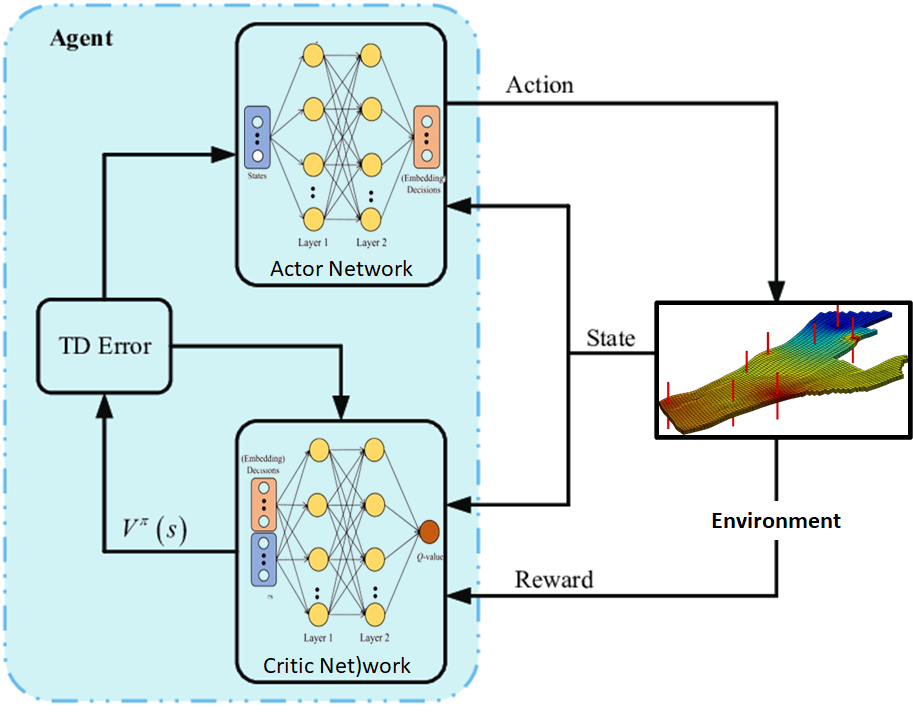
\includegraphics[width = \textwidth]{figures/prescriptive_analysis/a2c_process.png}
    \caption{Implementation of the actor critic architecture and its interaction with the environment}
    \label{fig:a2c_process}
\end{figure}

In this study, the agent can be inferred to represent an injector well. It provide the environment with actions that result in the optimal operating conditions for the simulated system. This agent is trained based on the net present value that is calculated using the feedback from the simulator. The agent used is an actor critic. 
The actor network represents a parameterized policy $(\pi_\theta)$. Hence, it is responsible for mapping states (st) to actions (at). The output of the actor’s network is a 3-dimensional vector representing the probability of the three actions. Those are increase, decrease and not changing in steam injection rate with reference to the previous injection rate. Then, using the probability distribution presented in Equation \ref{Eq:optimum_policy}, the action is determined. On the other hand, the critic network  evaluates the impact of actions by estimating the Q-value of a state-action pair. Hence, it takes both the state and the action as inputs. This ensures that the actor to critic agent consistently makes the best decision. 

\begin{equation}\label{Eq:optimum_policy}
    \pi_{\theta}\left(s,a\right) = \arg \max ⁡(\textbf{Softmax} P[ a|s,\theta])
\end{equation}

The actor agent is trained through the policy gradient method and optimized policy parameters are obtained through iterations. Equations \ref{Eq:gradient_cost} and \ref{Eq:theta_update} show the policy gradient cost function and parameters update.

\begin{equation}\label{Eq:gradient_cost}
    \mathrm{\nabla}_\theta\ J\left(\theta\right)=\ \mathrm{\nabla}_\theta{log}_{\pi_\theta}(a|s)V^{\pi_\theta}(S_t)	
\end{equation}
			
\begin{equation}\label{Eq:theta_update}
    \theta_{t+1}=\ \theta_t+\alpha\ \mathrm{\nabla}_\theta\ J\left(\theta\right)\ 
\end{equation}

Combining Equations (\ref{Eq:gradient_cost} and \ref{Eq:theta_update}) with the value function equation \ref{Eq:value_function} results in Equation \ref{Eq:theta_update_general}

\begin{equation}\label{Eq:value_function}
V_\pi(S)=\ \sum_{a\in A}{\pi\left(a,s\right)(R_s^a+\gamma\sum_{s^\prime\epsilon\ S} T_{ss\prime}^aV^\pi(s^\prime))}	    
\end{equation}

\begin{equation}\label{Eq:theta_update_general}
    \theta_{t+1}=\ \theta_t+\alpha\left[\ \mathrm{\nabla}_\theta{log}_{\pi_\theta}\left(a\middle| s\right)\sum_{a\in A}\pi\left(a,s\right)\left(R_s^a+\gamma\sum_{s^\prime\epsilon\ S} T_{ss^\prime}^aV^\pi\left(s^\prime\right)\right)\ \right]
\end{equation}

Such a technique exhibit high variance, since trajectories can lead to different returns. This is mainly due to stochasticity of the environment (random events during episode) and stochasticity of the policy. For instance, the same starting state can lead to very different returns. Because of this, the return at a specific point starting from the same state can vary significantly across episodes.

During iterations, the trajectory update was observed to have a high variance due to stochasticity of the environment and stochasticity of the policy. For instance, the same starting state can lead to different returns. Therefore, the return starting at the same state can vary significantly across episodes. The solution to mitigate the aforementioned problem is the usage of an advantage function Equation \ref{Eq:advantage_function}. The advantage function captures the degree of importance an action has compared to others for a given state, while the value function judges the strength of the decision.

\begin{equation}\label{Eq:advantage_function}
    A^{\pi_\theta}\left(S,a\right)=\ Q^{\pi_\theta}\left(S,\ a\right)-V^{\pi_\theta}\left(S\right)=r\left(a_t,S_t\right)+\gamma{\ V}^{\pi_\theta}\left(S_{t+1}\right)-V^{\pi_\theta}\left(S\right)
\end{equation}

Using Equation \ref{Eq:theta_update_general} and \ref{Eq:advantage_function} we get equations of actor and critic weights update \ref{Eq:actor_update} and \ref{Eq:critic_update}

\begin{equation}\label{Eq:actor_update}
\theta_{t+1}=\ \theta_t+\alpha[\mathrm{\nabla}_\theta{log}_{\pi_\theta}\left(a\middle| s\right)A^{\pi_\theta}(S,\ a)]
\end{equation}

\begin{equation}\label{Eq:critic_update}
    W_{t+1}=\ W_t+\beta A[\mathrm{\nabla}_wV^{\pi_\theta}\left(S_t\right)]
\end{equation}

Figure \ref{fig:steam_psudo_code} presents pseudo code for the actor critic algorithm for the steam injection process. 

\begin{figure}
    \centering
    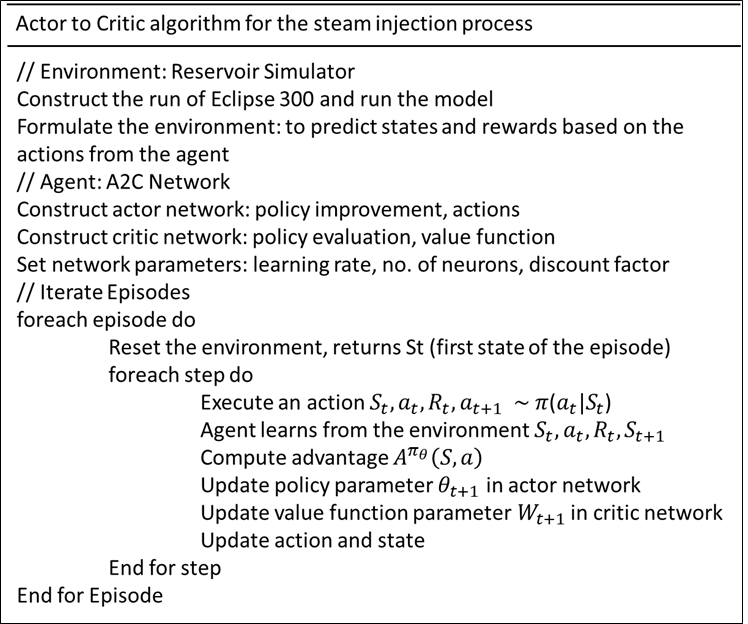
\includegraphics[width = \textwidth]{figures/prescriptive_analysis/steam_psudo_code.png}
    \caption{Pseudo code of the actor to critic algorithm for the steam injection process}
    \label{fig:steam_psudo_code}
\end{figure}

\section{Summary}
Steam injection is a common method to enhance the recovery from mature oil field. Commonly, a constant steam rate is applied over a long time without considering varying physical phenomena and reservoir characteristics, consequently resulting in a sub-optimal performance of these thermal heavy oil recovery processes. However, finding the optimal steam injection strategy is a challenge due to the complex dynamics, i.e., nonlinear formulation, variations over time and reservoir heterogeneity. Such a problem can be reformulated using the Markov decision process for the application of Reinforcement Learning (RL). Subsequently, a decision maker called Agent generate actions to maximize the production process yield. The agent do this by interacting continuously with the environment till reaches optimum route for injection rates.

In this work, an actor-critic RL architecture is used to train an agent to find the optimal strategy (i.e. policy) through interacting continuously with the environment. In this study, the environment is represented by a reservoir simulation model. At each time step, the agent executes an action by either increase, decrease or keep the steam injection rate constant and a subsequent reward is received by the agent. A reward can be defined as a distinct number from the environment. Then, the agent observes the new state from the environment. Such a state could be cumulative steam injected, pressure distribution or any other input that could be representative to the environment which is the reservoir simulation model in our case. During this interaction, a policy function and a value function are trained. A policy gives a probability distribution of the actions that the agent can take. For a specific policy, a value function determines the expected yield for an agent starting from a given state. This dynamic process executed for several episodes till convergence is achieved. 